\begin{frame}
\begin{center}
\Huge{Basemap and pyproj}
\end{center}
\end{frame}

\begin{frame}
\begin{center}
\Huge{Basemap}
\end{center}
\end{frame}

\begin{frame}
\frametitle{Basemap}
\begin{itemize}
  \item Matplotlib toolkit to plot maps
  \item Does provide facilities to convert coordinates to one of 25 map
  projections (using the PROJ library)
  \item Plotting is done by matplotlib
  \item Inbuild support for shapefiles
\end{itemize}
\end{frame}

\begin{frame}[fragile]
\frametitle{Basemap}
A very simple map:
\begin{myColorBox}{0.9}{}
\begin{verbatim}
>>> from mpl_toolkits.basemap import Basemap
>>> m = Basemap(projection='merc', llcrnrlat= 45.5, 
urcrnrlat=48, llcrnrlon=5, urcrnrlon=12, lat_ts= 47, 
resolution='i')
>>> m.drawcountries()
>>> plt.show()
\end{verbatim}
\end{myColorBox}
\pause
\begin{center}
      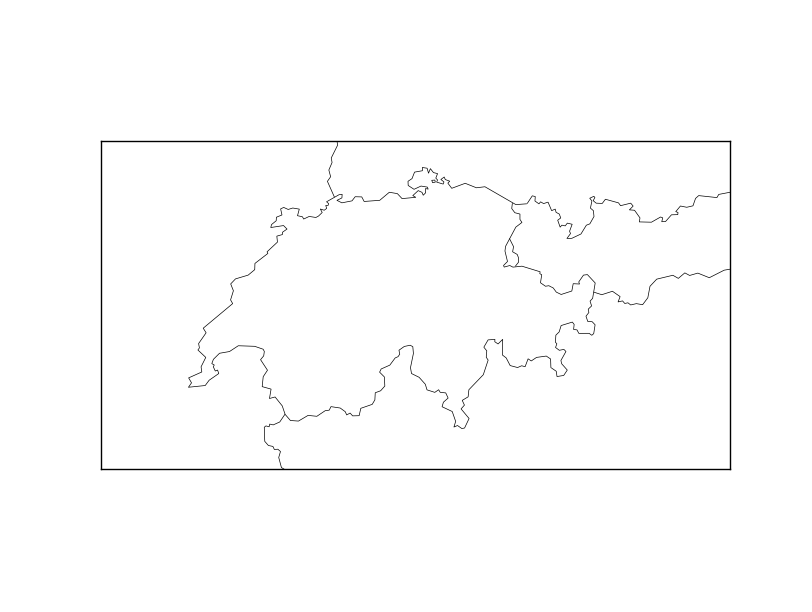
\includegraphics[width=0.8\textwidth]{pix/basemap_example_1}
\end{center}
\end{frame}

\begin{frame}[fragile]
\frametitle{Basemap}
\ldots adding a few details:
\begin{myColorBox}{1.0}{}
\begin{verbatim}
 >>> m.drawcoastlines()
 >>> m.drawcountries(linewidth=1.0)
 >>> m.drawmeridians([6,7,8,9,10,11],labels=[0,0,0,1])
 >>> m.drawparallels([46,46.5,47,47.5],labels=[1,0,0,0])
 >>> m.drawrivers(color='b')
 >>> plt.show()
\end{verbatim}
\end{myColorBox}
\pause
\begin{center}
      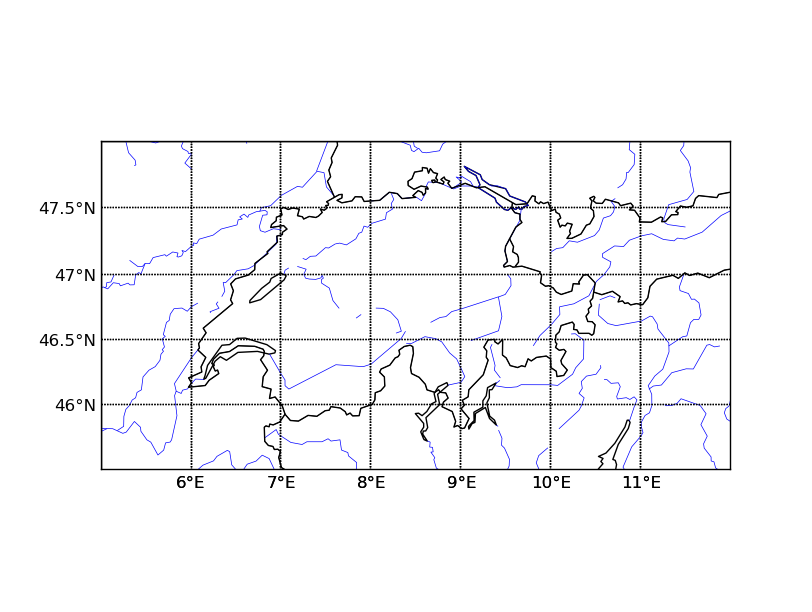
\includegraphics[width=0.8\textwidth]{pix/basemap_example_2}
\end{center}
\end{frame}
